% Packages

% Sets

% Formal statements


\begin{document}
\frame{\titlepage}

\begin{frame}{A goods distribution problem}
	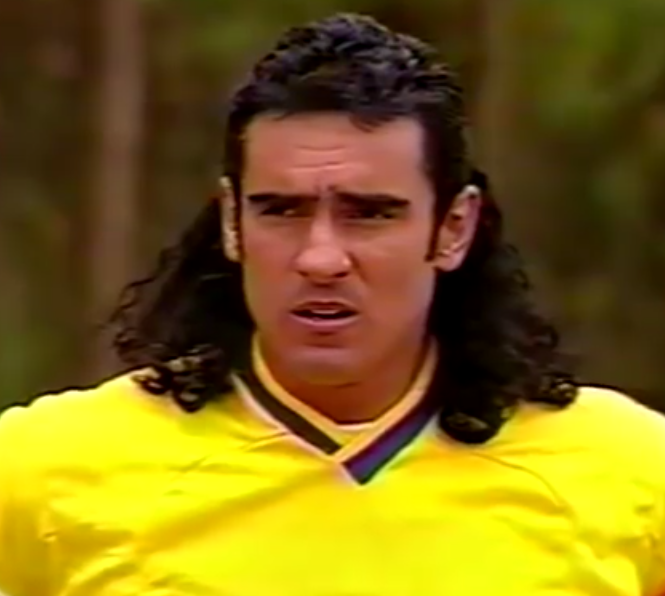
\includegraphics[width= 0.45\textwidth]{pedro_mirandoArco.png}
	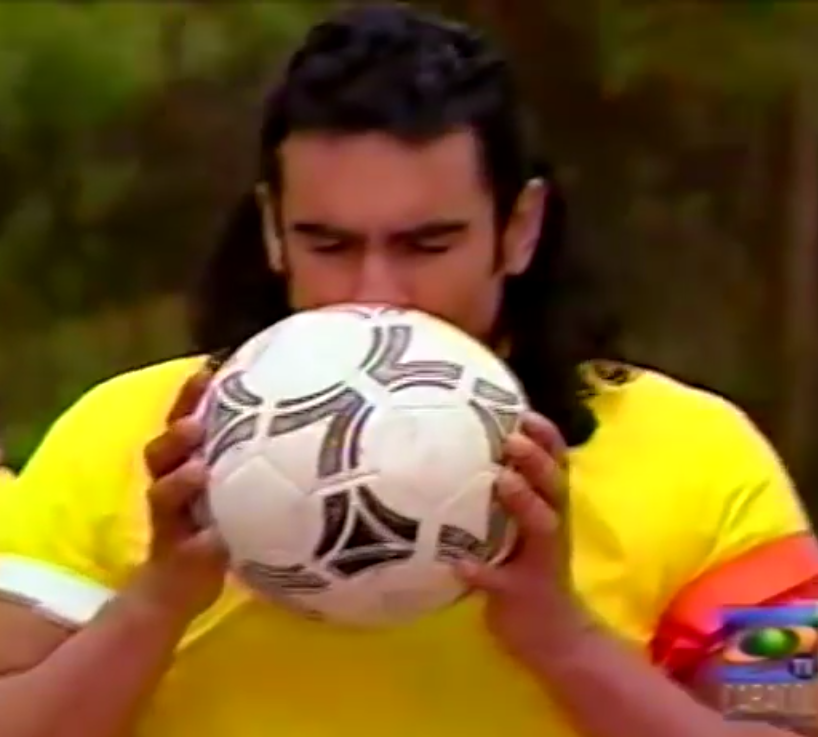
\includegraphics[width= 0.45\textwidth]{pedro_balon.png}
\end{frame}

%

\begin{frame}{A goods distribution problem}
	
\includegraphics[width= 0.25\textwidth]{balonGolty.png}
	\hspace{1cm}
	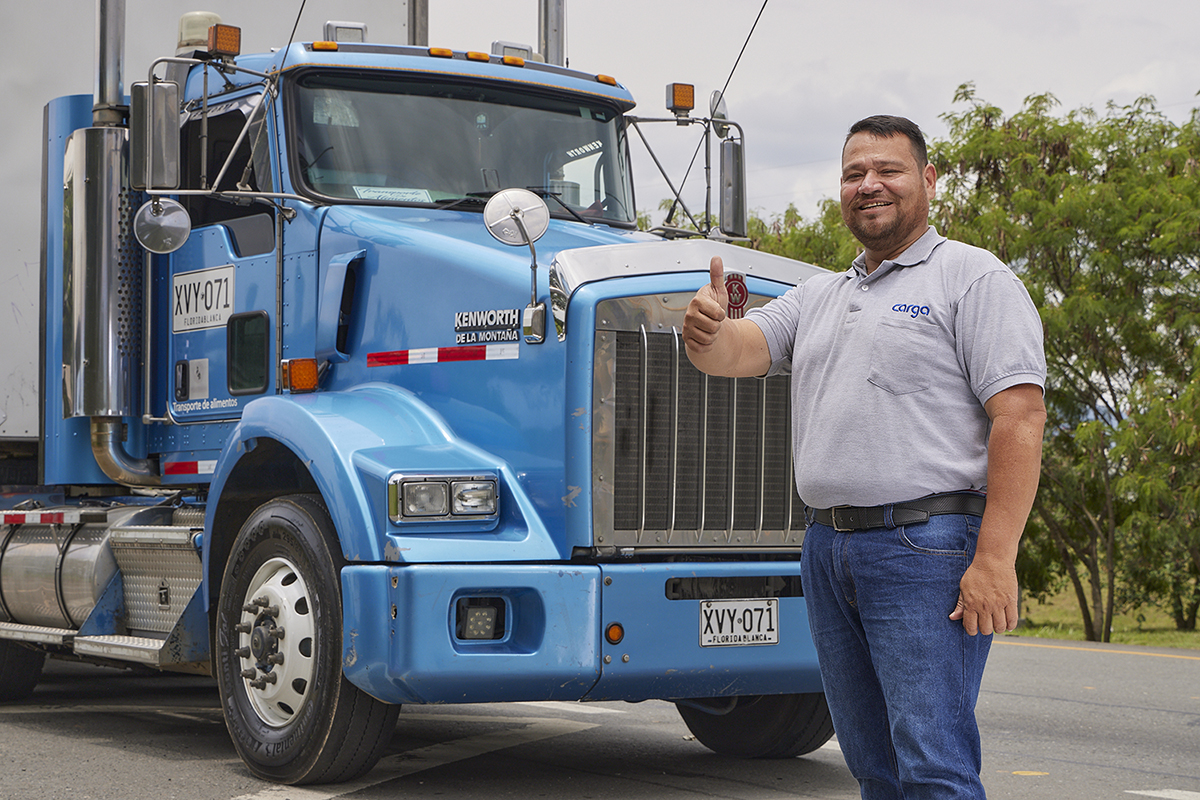
\includegraphics[width= 0.25\textwidth]{transporteDeCarga.jpg}

	\bigskip

	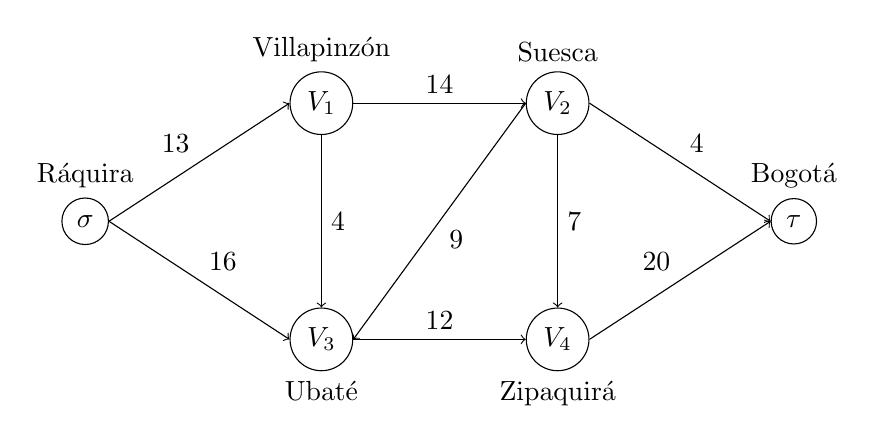
\begin{tikzpicture}
		\node[shape= circle, draw, label= above:Ráquira] (Raq) at (0,0) {$\sigma$};
		\node[shape= circle, draw, label= above:Villapinzón] (Vil) at (3,1.5) {$V_1$};
		\node[shape= circle, draw, label= above:Suesca] (Sue) at (6,1.5) {$V_2$};
		\node[shape= circle, draw, label= below:Ubaté] (Uba) at (3,-1.5) {$V_3$};
		\node[shape= circle, draw, label= below:Zipaquirá] (Zip) at (6,-1.5) {$V_4$};
		\node[shape= circle, draw, label= above:Bogotá] (Bog) at (9,0) {$\tau$};
		% Connections
		%% Non-crossing
		\draw [->] (Raq.east) to node [auto] {13} (Vil.west);
		\draw [->] (Vil.east) to node [auto] {14} (Sue.west);
		\draw [->] (Sue.east) to node [auto] {4} (Bog.west);
		\draw [->] (Raq.east) to node [auto] {16} (Uba.west);
		\draw [->] (Uba.east) to node [auto] {12} (Zip.west);
		\draw [->] (Zip.east) to node [auto] {20} (Bog.west);
		%% Crossing
		\draw [->] (Vil.south) to node [auto] {4} (Uba.north);
		\draw [->] (Sue.south) to node [auto] {7} (Zip.north);
		\draw [->] (Sue.west) to node [auto] {9} (Uba.east);
	\end{tikzpicture}
\end{frame}
\end{document}
